\chapter{The Hidden Markov model}

The definitions in this chapter are based on \cite[pp.~210]{jm09}, but use
different variable names in several places to avoid conflicts with the notation
from chapter~2.

\begin{definition}
 A \emph{Hidden Markov model} (HMM) is a quintuple\footnote{This definition
 diverges in structure from \cite{jm09} in one significant way: It uses a
 single state $\#$ instead of a pair of initial state $q_0$ and final state
 $q_F$. This allows us to use a single probability distribution $t$ to describe
 all state transitions, instead of the triple of matrices $(a_{0i})_i$,
 $(a_{ij})_{(i,j)}$, and $(a_{iF})_i$ that appear in \cite{jm09}.} $H =
 (Q,V,\#,t,e)$ such that
 \begin{itemize}\setlength\itemsep{-0.3em}
  \item $Q$ is a non-empty alphabet (of states),
  \item $V$ is a non-empty alphabet (of words),
  \item $\#\notin Q\cup V$ is a separate (initial and final) state,
  \item $t\in\um(Q\cup\brc{\#}|Q\cup\brc{\#})$ and $e\in\um(V|Q)$. \qedhere
 \end{itemize}
\end{definition}

From here on, we will abbreviate $Q\cup\brc{\#}$ as $Q_\#$.

The Hidden Markov model describes a sentence as being the result of the
progression of a probabilistic state machine that starts out in $\#$, traverses
states from $Q$, and in the end reaches $\#$ again. Each time a state from $Q$
is reached, a word from $V$ is emitted. The sequence of all these emitted words
is the sentence that is observed.

When a sentence $v = v_1\cdots v_n\in V^+$ is observed, is must have been
caused by a certain sequence of states $q = q_1\cdots q_n\in Q^*$, but it is
not known which one it was, only that the lengths of both sequences agree.
Therefore, by the law of total probability,
\[
 P(v) = \sum_{q\in Q^n} P(v|q) \cdot P(q).
\]

%TODO find a reference for "Markov property" (this paragraph is currently more
%or less copied from en.wikipedia)
\begin{definition}
 A stochastic process is said to have the \emph{Markov property} if the
 conditional probability distribution of future states of the process only
 depends on the present state, not on the states before or after it.
\end{definition}

A Hidden Markov model exhibits the Markov property in two separate ways: First,
the conditional probability distribution of each state depends only on the
state directly preceding it. Second, the conditional probability distribution
of each emitted word depends only on the state that was inhabited at the time
of emission. These two conditional probability distributions are called $t$ and
$e$, and are part of the quintuple $H=(Q,V,\#,t,e)$ as defined before.

The progression of the probabilistic state machine of $H$ through the state
sequence $q=q_1\cdots q_n$ involves several separate stochastic events:
entering each state $q_1,\ldots,q_n$ in that order, then entering the state
$\#$ after $n$ other states. Therefore, by the chain rule,
\[
 P(q_1\cdots q_n) = P(q_1,\ldots,q_n,n) = P(q_1) \cdot P(q_2|q_1) \cdots P(q_n|q_1,\ldots,q_{n-1}) \cdot P(n|q_1,\ldots,q_n).
\]
The last factor, $P(n|q_1,\ldots,q_n)$ is the probability of the state sequence
having length $n$ if $q_1,\ldots,q_n$ are known or, in other words, the
probability of the state sequence terminating (by the state machine coming back
to $\#$) after these $n$ states. Since, by the first Markov property, each
state only depends on the one directly preceding it, we can reformulate each
factor in terms of the conditional probability distribution $t$:
\begin{align*}
 P(q_1) &=: t(q_1|\#), \\
 P(q_i|q_1,\ldots,q_{i-1}) &= P(q_i|q_{i-1}) =: t(q_i|q_{i-1}), \\
 P(n|q_1,\ldots,q_n) &= P(n|q_n) =: t(\#|q_n),
\end{align*}
and therefore,
\[
 P(q_1\cdots q_n) = t(q_1|\#) \cdot t(q_2|q_1) \cdots t(q_n|q_{n-1}) \cdot t(\#|q_n).
\]

In a similar way, we can rewrite $P(v|q)$ as
\[
 P(v_1\cdots v_n|q_1\cdots q_n) = \prod_{i=1}^n P(v_i|q_1\cdots q_n)
\]
and codify the second Markov property as
\[
 P(v_i|q_1\cdots q_n) = P(v_i|q_i) =: e(v_i|q_i).
\]

Putting all these results into the original equation for $P(v)$, we obtain
\[
 P(v=v_1\cdots v_n) = \sum_{q_1,\ldots,q_n} t(q_1|\#) \cdot e(v_1|q_1) \cdot \prod_{i=2}^n \mbig\brk{t(q_i|q_{i-1}) \cdot e(v_i|q_i)} \cdot t(\#|q_n).
\]

\section{Forward and backward algorithms}

When $P(v)$ is computed in this manner, the computation takes an exponential
amount of time in the sentence length $n$ since $\abs Q^n$ summands need to be
evaluated. However, for similar state sequences, some subterms can be reused
across summands, thereby reducing the required computation effort. There are
two standard schemes for this, the \emph{forward algorithm} and the
\emph{backward algorithm}.

\begin{definition}
 Let $H=(Q,V,\#,t,e)$ be an HMM, $q\in Q$ be a state, $v=v_1\cdots v_n\in V^+$
 be a sentence, and $i\in\brc{1,\ldots,n}$.\footnote{\cite{jm09} uses the
 term ``time'' and the symbol $t$ for this index. We avoid the symbol $t$
 because it is already used for the transition probability.} The \emph{forward
 weight}\footnote{The names ``forward/backward weight'' have been chosen
 deliberately, because we will see in the next section that these values
 correspond to the inside and outside weight.} $T_v(i,q)$ is the probability
 of the HMM being in state $q$ after having emitted the first $i$ words of
 $v$. The \emph{backward weight} $S_v(i,q)$ is the probability of the HMM
 generated $v$ when the first $i$ words of $v$ have already been generated and
 the HMM is in state $q$ after that many words.
\end{definition}

The forward weight can be calculated by following the same methods as in the
previous section for $P(v)$. For $i = 1$, the forward weight describes the
transition from the initial state $\#$ into $q$, and the emission of $v_1$ in
that state:
\[
 T_v(1,q) = P(v_1,q_1=q) = P(q_1=q) \cdot P(v_1|q_1=q) = t(q|\#) \cdot e(v_1|q).
\]
For $i\geq 2$, the forward weight can be calculated iteratively by first
obtaining the forward weights $T_v(i-1,q')$ for any possible previous state
$q'\in Q$, because
\[
 T_v(i,q) = P(v_1,\ldots,v_i,q_i=q) = \sum_{q'\in Q} P(v_1,\ldots,v_i,q_{i-1}=q',q_i=q)
\]
by the law of total probability, and then, by the chain rule and the Markov
properties of the HMM,
\begin{align*}
 T_v(i,q)
  &= \sum_{q'\in Q} P(v_1,\ldots,v_{i-1},q_{i-1}=q') \cdot P(q_i=q|q_{i-1}=q') \cdot P(v_i|q_i=q) \\
  &= \sum_{q'\in Q} T_v(i-1,q') \cdot t(q|q') \cdot e(v_i|q) \\
  &= e(v_i|q) \cdot \sum_{q'\in Q} T_v(i-1,q') \cdot t(q|q').
\end{align*}
The probability $P(v)$ can then be computed in a similar way as
\[
 P(v) = P(v_1,\ldots,v_n,n) = \sum_{q\in Q} P(v_1,\ldots,v_n,q_n=q) \cdot P(n|q_n=q) = \sum_{q\in Q} T_v(n,q) \cdot t(\#|q).
\]
In order to compute $P(v)$, the full matrix of $\mbig\kla{T_v(i,q)}_{i,q}$ must
be computed. Each of these forward weights can be computed in $O\mbig\kla{\abs
Q}$ time because $\abs Q$ summands need to be added. Therefore, $P(v)$ can be
computed in $O\mbig\kla{n \cdot \abs Q^2}$ time, which is much better than the
exponential time required for the initial formula for $P(v)$.

The same time complexity arises when $P(v)$ is being restated in terms of
backward weights. Backward weights can be computed in a similar manner to
forward weights, with the difference of iterating in opposite temporal order.
\begin{align*}
 P(v) &= \sum_{q\in Q} t(q|\#) \cdot e(v_1|q) \cdot S_v(1,q) \\
 \text{where } S_v(i,q) &= \begin{cases}
  t(\#|q) & \text{if }i=n, \\
  \sum_{q'\in Q} t(q'|q) \cdot e(v_{i+1}|q') \cdot S_v(i+1,q') & \text{otherwise}.
 \end{cases}
\end{align*}

\section{The Baum-Welch algorithm}

\begin{algorithm}[p!]
 \caption{Baum-Welch algorithm, based on \cite[p.~226]{jm09}. To reach a local
 maximum (or saddle point) for the corpus likelihood $p(c)$, the outermost loop
 needs to be executed until $(t,e)$ stop changing, possibly infinitely long.
 The loop condition is stated as ``not converged'' to capture that the loop is
 typically aborted once the changes to $(t,e)$ per iteration fall below some
 manually chosen threshold.\\[1em]
 The formulation of the algorithm has been altered from \cite{jm09} to also
 train the transition probabilities for the initial and final state, and to
 support a corpus with multiple sentences of different length (by taking sums
 over the time index $i$ in the E-step rather than in the M-step). The same
 alterations have already been successfully applied to an implementation of HMM
 in \cite{nel13}. \label{alg:bw-vogler}}
 \begin{algorithmic}[1]
  \algorithmheader[Input:] HMM $H_0 = (Q,V,\#,t_0,e_0)$; $V^+$-corpus $h$
  \algorithmheader[Variables:] $t:\um(Q_\#|Q_\#)$, $e:\um(V|Q)$
  \algorithmheader             $\cnt_\mathrm{tr}: Q_\#\times Q_\#\to\zr_{\geq0}$
  \algorithmheader             $\cnt_\mathrm{em}: V\times Q\to\zr_{\geq0}$
  \algorithmheader[Output:] HMM $H = (Q,V,\#,t,e)$
  \algorithmheader such that $p_H(c) \geq p_{H_0}(c)$ and $H$ maximizes $p_H(c)$ locally
  \STATE $(t,e) \leftarrow (t_0,e_0)$
  \WHILE{not converged}
   \STATE consider the HMM $(Q,V,\#,t,e)$
   \STATE $\cnt_\mathrm{tr}(q,q') \leftarrow 0$ \SUFFIXFOR{$q,q'\in Q_\#$}
   \STATE $\cnt_\mathrm{em}(w,q) \leftarrow 0$ \SUFFIXFOR{$q\in Q$ and $w\in V$}
   \FOR{$v=v_1\cdots v_n\in\operatorname{supp}(h)$}
    \STATE calculate all forward weights $T_v(i,q)$ and backward weights $S_v(i,q)$
    \FOR{$i=1,2,\ldots,n-1$}
     \FOR{$q,q'\in Q$}
      \STATE $\cnt_\mathrm{tr}(q,q') \leftarrow \cnt_\mathrm{tr}(q,q') + h(v) \cdot U_v(i,q',q)$
     \ENDFOR
    \ENDFOR
    \FOR{$i=1,2,\ldots,n$}
     \FOR{$q\in Q$}
      \STATE $\cnt_\mathrm{em}(v_i,q) \leftarrow \cnt_\mathrm{tr}(v_i,q) + h(v) \cdot R_v(i,q)$
     \ENDFOR
    \ENDFOR
    \FOR{$q\in Q$}
     \STATE $\cnt_\mathrm{tr}(q,\#) \leftarrow \cnt_\mathrm{tr}(q,\#) + h(v) \cdot R_v(1,q)$
     \STATE $\cnt_\mathrm{tr}(\#,q) \leftarrow \cnt_\mathrm{tr}(\#,q) + h(v) \cdot R_v(n,q)$
    \ENDFOR
   \ENDFOR
   \FOR{$q,q'\in Q_\#$}
    \STATE $t(q|q') \leftarrow \frac{\cnt_\mathrm{tr}(q,q')}{\sum_{q''} \cnt_\mathrm{tr}(q'',q')}$
   \ENDFOR
   \FOR{$q\in Q$ and $w\in V$}
    \STATE $e(w|q) \leftarrow \frac{\cnt_\mathrm{em}(w,q)}{\sum_{w'} \cnt_\mathrm{em}(w',q)}$
   \ENDFOR
  \ENDWHILE
 \end{algorithmic}
\end{algorithm}

The Baum-Welch algorithm is first stated in \cite{baupetsouwei70}, but since
notational conventions have changed considerably since then, we are going to
use a contemporary formulation in \cite{jm09} as a reference (see
Algorithm~\ref{alg:bw-vogler} on page~\pageref{alg:bw-vogler}).

The algorithm uses two terms that have not yet been introduced: $U_v(i,q',q)$ is
defined as the probability of the HMM progressing from state $q'$ into state
$q$ at time $i+1$ while generating the sentence $v$. $R_v(i,q)$ is the probability
of the HMM being in state $q$ at time $i$ while generating the sentence $v$.
\begin{align*}
 U_v(i,q',q) &:= P(q_i = q',q_{i+1} = q|v) && \text{for } i\in\brc{1,\ldots,\abs v-1}, q,q'\in Q \\
 R_v(i,q) &:= P(q_i=q|v) && \text{for } i\in\brc{1,\ldots,\abs v},q\in Q
\end{align*}

Both $U_v$ and $R_v$ can be expressed in terms of the forward and backward weights
$T_v$ and $S_v$, by applying the same calculation rules for probabilities that were
already used for deriving the formulas for $P(v)$, $T_v$ and $S_v$.
\begin{align*}
 R_v(i,q)
  &= P(q_i=q|v) = \frac{P(v_1,\ldots,v_n,n,q_i=q)}{P(v)} \\
  &= \frac{P(v_1,\ldots,v_i,q_i=q) \cdot P(v_{i+1},\ldots,v_n,n|q_i=q)}{P(v)} \\
  &= \frac{T_v(i,q) \cdot S_v(i,q)}{P(v)}
\end{align*}

And analogously,
\begin{align*}
 U_v(i,q',q)
  &= P(q_i = q',q_{i+1} = q|v) = \frac{P(v_1,\ldots,v_n,n,q_i=q',q_{i+1}=q)}{P(v)} \\
  &= \frac1{P(v)} \cdot \brk{\begin{matrix}
   P(v_1,\ldots,v_i,q_i=q') \cdot P(q_{i+1}=q|q_i=q') \\
   \cdot\; P(v_{i+1}|q_{i+1}=q) \cdot P(v_{i+2},\ldots,v_n,n|q_{i+1}=q)
  \end{matrix}} \\
  &= \frac{T_v(i,q') \cdot t(q|q') \cdot e(v|q) \cdot S_v(i+1,q)}{P(v)}.
\end{align*}

\section{Deriving the Baum-Welch algorithm}

\cite{jm09} describes Baum-Welch as an instance of the EM algorithm. And
indeed, the basic structure of the algorithm looks similar to the types of EM
algorithms that we have introduced in chapter 2 in several ways:
\begin{itemize}
 \item $t$ and $e$ are the model parameters that are iteratively optimized.
 \item $\cnt_\mathrm{tr}$ and $\cnt_\mathrm{em}$ act like complete-data
  corpora. They are computed using the previous model parameters, then new
  model parameters are obtained by taking the empirical probability
  distribution of these corpora, which is the efficient solution to the
  conditional maximum-likelihood estimator that is suggested by
  Lemma~\ref{lemma:empirical2}.
 \item The hidden information is the state sequence $q$ that produces the
  sentence $v$ from the corpus. It can be destructured into countable events in
  several ways (e.~g.~states only, pairs of time and states, or pairs of
  subsequent states).
 \item The way that forward weights and backward weights appear in the
  computation of $\cnt_\mathrm{tr}$ and $\cnt_\mathrm{em}$ is similar to how
  inside and outside weights appear in the computation of the inside-outside
  complete-data corpus.
\end{itemize}

Therefore, in the remainder of this chapter, we will show that the Baum-Welch
algorithm can be obtained from the generic EM algorithm from chapter~2 through
suitable instantiation of the inside-outside step mapping.

\subsection{Model parameter and countable events}

For the remainder of this section, let $H = (Q,V,\#,t,e)$ be an HMM.
Observations are sentences with words from $V$, i.~e.,
\[
 X = V^+.
\]

An IO information contains only one component which can be subject to training:
the model parameter $\omega$ which chooses the conditional probability
distribution
\[
 q_\omega \in \um_C(A|B).
\]

For a HMM, $q_\omega$ must describe both the transmission and emission
probability. We therefore choose
\[
 \Omega := \um(Q_\#|Q_\#) \times\um(V|Q)
\]
such that every model parameter $\omega=(t,e)$ is a pair of transition and
emission probability for~$H$. Moreover, we choose
\begin{align*}
 A &:= Q_\#\cup V, \\
 B &:= Q_\# \times \brc{E,T}, \\
 C &:= \mbig\brc{\mbig\kla{q',(q,T)}\mid q,q'\in Q_\#} \cup \mbig\brc{\mbig\kla{v,(q,E)}\mid v\in V, q\in Q}, \\
 q_{\omega=(t,e)}\mbig\kla{a\!\dmiddle|\!(q,b)} &:= \begin{cases}
  t(a|q) & \text{if } b = T \text{ and } a\in Q_\#, \\
  e(a|q) & \text{if } b = E \text{ and } a\in V \text{ and } q \neq\#, \\
  1 & \text{if } b = E \text{ and } a = q = \#, \\
  0 & \text{otherwise.}
 \end{cases}
\end{align*}

Herein, $E$ and $T$ are symbols such that $E,T\notin Q\cup V$ that denote if a
countable event $c\in C$ is a transition event
\[
 c = \mbig\kla{q',(q,T)} \text{ with probability } q_{(t,e)}(c) = t(q'|q).
\]
or an emission event
\[
 c = \mbig\kla{v,(q,E)} \text{ with probability } q_{(t,e)}(c) = e(v|q).
\]

The choice of $q_\omega\mbig\kla{\#\!\dmiddle|\!(\#,E)}=1$ as above ensures that
$q_\omega\in\um_C(A|B)$ for all $\omega=(t,e)$.

\begin{proof}
 Let $\omega=(t,e)\in\Omega$. It is easy to see that
 $\operatorname{supp}(q_\omega)\subseteq C$ since $q_\omega(a|b)$ was defined
 as 0 for any $c\notin C$. According to Definition~\ref{def:02-cpd}, what
 remains to be shown is that $q_\omega\mbig\kla{(q,b)}\in\um(A)$ for every
 $(q,b)\in B$. For $q\in Q_\#$ and $b = T$,
 \[
  \sum_{a\in A} q_{(t,e)}\mbig\kla{q'\!\dmiddle|\!(q,T)} = \sum_{q'\in Q_\#} q_{(t,e)}\mbig\kla{q'\!\dmiddle|\!(q,E)} = \sum_{q'\in Q_\#} t(q'|q) = 1
 \]
 because $t\in\um(Q_\#|Q_\#)$. Analogously, for $q\in Q$ and $b = E$, we have
 \[
  \sum_{a\in A} q_{(t,e)}\mbig\kla{a\!\dmiddle|\!(q,E)} = \sum_{v\in V} q_{(t,e)}\mbig\kla{v\!\dmiddle|\!(q,E)} = \sum_{v\in V} e(v|q) = 1
 \]
 because $e\in\um(V|Q)$. It remains to see that
 \[
  \sum_{a\in A} q_\omega\mbig\kla{a\!\dmiddle|\!(\#,E)} = 1,
 \]
 which is ensured by the only nonzero contribution to this sum being
 $q_\omega\mbig\kla{\#\!\dmiddle|\!(\#,E)} = 1$.
\end{proof}

It shall be noted that the countable event $\mbig\kla{\#,(\#,E)}$ is only used
to ensure $q_\omega\in\um_C(A|B)$. It does not appear in any $y\in Y$.

\subsection{Tree-shaped hidden information}

\begin{figure}[t!]
 \centering
 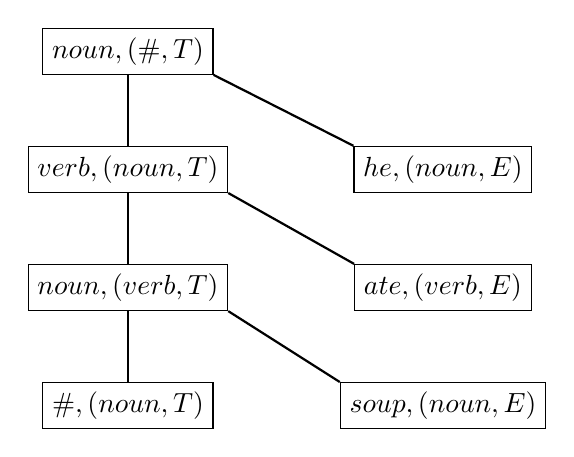
\begin{tikzpicture}[every node/.style={rectangle,draw}]
  \node(t0) at (0,0) { $\text{noun},(\#,T)$ };
  \node(t1) at (0,-1.5) { $\text{verb},(\text{noun},T)$ } edge[thick] (t0);
  \node(t2) at (0,-3.0) { $\text{noun},(\text{verb},T)$ } edge[thick] (t1);
  \node(t3) at (0,-4.5) { $\#,(\text{noun},T)$ }          edge[thick] (t2);
  \node(e1) at (4,-1.5) { $\text{he},(\text{noun},E)$ };
  \node(e2) at (4,-3.0) { $\text{ate},(\text{verb},E)$ };
  \node(e3) at (4,-4.5) { $\text{soup},(\text{noun},E)$ };
  \draw[thick] (t0.south east) -- (e1.north west);
  \draw[thick] (t1.south east) -- (e2.north west);
  \draw[thick] (t2.south east) -- (e3.north west);
 \end{tikzpicture}
 \caption{Example for a hidden information $y\in Y\subseteq T_C$ corresponding
 to the observation $x = \text{``He ate soup.''}$ and the state sequence
 ``noun-verb-noun''.\label{fig:03-example-y}}
\end{figure}

In order to describe hidden information $y\in Y$ as a ranked tree of countable
events from $C$, we assign a rank to each $c = \mbig\kla{a,(q,b)}\in C$ as follows:
\begin{align*}
 \rk\mbig\kla{a,(q,b)} := \begin{cases}
  0 & \text{if } b = E, \\
  2 & \text{if } b = T \text{ and } q\neq\#, \\
  0 & \text{if } b = T \text{ and } q = \#.
 \end{cases}
\end{align*}

The intuition for this choice is that each transition event causes two further
events: the emission event in the state that was entered, and the transition
event into the state after that. Emission events do not result in further
events because of the Markov property, and a transition event into the $\#$
state marks the end of the stochastic process after which no further events
occur. This rank assignment results in trees such as the one in
Figure~\ref{fig:03-example-y}.

The trees $y\in Y$ are generated by the tree grammars $H(x)$ and $K$. We define
\[
 K := \mbig\brc{Q_K, (\#,0,T), R_K} \quad\text{where}\quad Q_K = Q_\# \times \zn \times \brc{E,T}
\]
and $R_K$ contains the following rules:
\begin{align*}
 (\#,0,T) &\to \mbig\kla{q,(\#,T)}\mbig\kla{(q,1,T),(q,1,E)} &&\forall q\in Q, \\
 (q,i,T) &\to \mbig\kla{q',(q,T)}\mbig\kla{(q',i+1,T),(q',i+1,E)} &&\forall q,q'\in Q \text{ and } i\geq1, \\
 (q,i,T) &\to \mbig\kla{\#,(q,T)} &&\forall q\in Q\text{ and } i\geq 1, \\
 (q,i,E) &\to \mbig\kla{v,(q,E)} &&\forall q\in Q\text{ and } i\geq 1 \text{ and } v\in V.
\end{align*}

The IO information requires that $K$ is unambiguous. It is easy to see that
this is the case: $K$ is deterministic because each $c\in C$ is produced by at
most one rule from $R_K$, and all deterministic RTG are also unambiguous
(see~page~\pageref{lemma:02-deterministic-is-unambiguous}).






{\color{red}TODO: $H(x)$, $\pi_1$, $Y$ as $\sum_x \pi_1^{-1}(x)$; $\alpha$, $\beta$, $\chi$, $c\dangle{\omega,\mu}$, $\stepmap\mu_\mathrm{io}$}
